\chapter{Bewertung verschiedener Methoden}
\label{ch:bewertung}

Nachfolgend werden die verschiedenen Arten von CAPTCHA sowie einige Alternativen auf Basis der zuvor entwickelten Matrix bewertet. 
Dafür wird sich an den in Kapitel \ref{ch:matrix} aufgestellten Leitfragen soweit möglich orientiert.

\section{Textbasierte CAPTCHA}
\label{ch:bewertung:text}
Durch ihren simplen Aufbau sind textbasierte CAPTCHAs relativ einfach zu verstehen.
Es sind wenige Clicks nötig, um einen solchen CAPTCHA auszufüllen. 
Bei optisch verzerrten Wörtern besteht jedoch die Möglichkeit, dass es zu Missverständnissen kommen kann.
So können beispielsweise ein kleines ``d'' und ein ``cl'' unter Umständen auch von Menschen verwechselt werden. 
In \autoref{fig:schwierig} ist ein ähnlicher Fall dargestellt. 
Wenn man sich nicht bewusst ist, dass hier nur korrekte Wörter der englischen Sprache erfragt werden,
kann das zweite Wort (``blotch'') auch als ``bbtch'' interpretiert werden. (Vgl. \cite[p.132]{Beheshti})

\begin{figure}[h!]
    \centering
    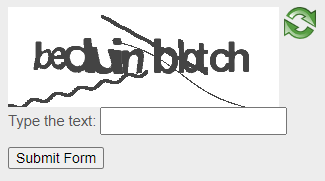
\includegraphics[width=6cm]{gfx/mygraphics/schwierig4.png}
    \caption{Textbasierter CAPTCHA aus der Securimage phpCaptcha Demo, welcher nicht eindeutig zu beantworten ist}
    \label{fig:schwierig}
\end{figure}

Damit würde der CAPTCHA nicht korrekt beantwortet werden können.
Da dies oft bei dieser CAPTCHA-Art vorkommt, kann bei der Bedienfreundlichkeit keine volle Punktzahl gegeben werden,
sondern es müssen je nach Komplexität ein bis zwei Punkte abgezogen werden.

Zeitliche Begrenzungen können vorkommen, sind aber nicht bei jeder Technik anzutreffen.
Hier ist, sofern gegeben, ebenfalls ein Punkt abzuziehen.

Accessability ist ambivalent zu betrachten.
Textbasierte CAPTCHA allein sind für sehbehinderte Menschen nicht nutzbar. 
Da dies eine Personengruppe vollständig ausschließt, werden zwei Punkte abgezogen.

Ebenso können die verschiedenen Techniken, die bei textbasierten CAPTCHAs angewandt werden, zu Problemen für Legastheniker führen.
Auch Menschen mit Farbfehlsichtigkeiten können durch eine Kombination von ungünstig generierten Hintergründen und Schriftfarben irritiert werden.
Aus diesem Grund wird auch hier jeweils ein Punkt abgezogen.

Einige textbasierte CAPTCHAs lassen sich gut audiobasiert umsetzen, 
um die Accessibility des CAPTCHAs zu gewährleisten. 
Dies führt somit nicht zu einem Punktabzug.

Die technische Umsetzbarkeit ist bei verschiedenen betrachteten Techniken zur Erstellung und Nutzung textbasierter CAPTCHAs sehr simpel gehalten.
Die Dokumentation ist gut und kann über Programmierschnittstellen (APIs) leicht eingebunden werden. (Vgl. \cite{hcaptcha} \cite{phpcaptcha} \cite{reallysimplecaptcha})
Aus diesem Grund kann hier die volle Punktzahl vergeben werden.

\citeauthor{surveyofresearch} schreiben in \citetitle{surveyofresearch}, 
dass Hollow CAPTCHA durch eine Kombination von Segmentierung und Recognition %TODO
mit einer Erfolgsrate von 36 bis 89 Prozent durch Bots gelöst werden konnten. (Vgl. \cite[p.76ff]{surveyofresearch}) %TODO

Ähnlich verhält es sich bei Überlappungen und CCT (``crowing characters together''):
Hier konnte bei verschiedenen Technologien mithilfe von unterschiedlichen Methoden
eine Erfolgsquote von 27,1 bis 53,2 Prozent erreicht werden. \cite[p.76]{surveyofresearch} %Quellen aus Text noch mit aufnehmen

Auch bei ``noise backgrounds'' und ``two-layer structures'' konnten solche Ergebnisse erzielt werden. 
(Vgl. \cite[p.76]{surveyofresearch})
Da es bereits viele sehr erfolgreiche Methoden gibt, um diese Art der CAPTCHAs durch Bots absolvieren zu lassen,
werden 5-7 Punkte im Kontext Sicherheit abgezogen. 

Auf Basis dieser Erkenntnisse werden textbasierte CAPTCHAs wie in Tabelle \ref{table:matrix:text} bewertet.

%Multifonts, Rotation, Waving, Large character set \cite{surveyofresearch}

\begin{table}[h!]
    \caption{Bewertungsmatrix für textbasierte CAPTCHAs}
    \begin{center}
        \begin{tabular}{l|c}
            Kategorie                       & Bewertung \\\hline
            Bedienfreundlichkeit            & 7-9         \\
            Accessibility                   & 6-10        \\
            Technische Umsetzbarkeit        & 10         \\
            Sicherheit                      & 3-5         
        \end{tabular}
    \end{center}
    \label{table:matrix:text}
\end{table}

\section{Bildbasierte CAPTCHA}
\label{ch:bewertung:bild}
Bildbasierte CAPTCHAs benötigen etwas mehr Aufwand als beispielsweise textbasierte CAPTCHAs.
Je nach verwendeter Technik muss auf eine Reihenfolge geachtet werden. 
Es ist auch möglich, dass bei einigen Bildern genau darauf geachtet werden muss, ob die gegebenen Antworten wirklich korrekt sind.
In \autoref{fig:fortnite} (a) ist beispielsweise nur schwer zu erkennen, ob manche Hunde wirklich geschlossene Augen haben, 
oder ob der Kontrast zwischen Fell und Iris lediglich zu gering ist.

\begin{figure}[h!]
    \centering
    \subfloat[\centering]{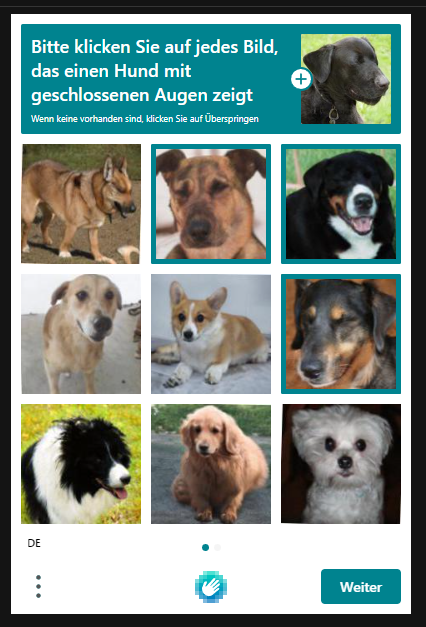
\includegraphics[width=6cm]{gfx/mygraphics/fuerfortnite.png}}
    \subfloat[\centering]{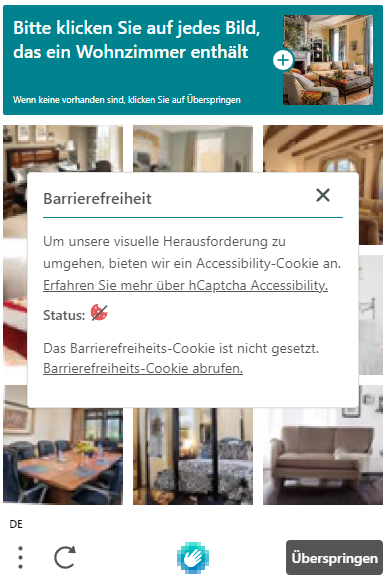
\includegraphics[width=6cm]{gfx/mygraphics/barrierefreiheit.png}}
 \caption{Bildbasierter CAPTCHA von hCaptcha bei Login auf der Epic Games Website (a) und barrierefreie Alternative von hCaptcha (b)}
      \label{fig:fortnite}
\end{figure}

Bei sehr detailreichen Bildern kann es vorkommen, dass auch ein Mensch mehrere Versuche benötigt, da eventuell nicht jedes gesuchte Objekt sofort erkannt wird.

Deshalb werden bei sehr hoher Komplexität oder bei schwer zu erkennenden Bildern zwischen 2 und 4 Punkte bei der Bedienfreundlichkeit abgezogen.
Bei bildbasierten CAPTCHAs kommen bemerkbare zeitliche Begrenzungen eher selten vor. 

Auch hier besteht die Problematik, dass Menschen mit eingeschränker Sicht keine Chance haben, diese Art von CAPTCHAs adäquat auszufüllen.
Es gibt teilweise die Möglichkeit, eine audiobasierte Alternative anzubieten. 
So wird es beispielsweise bei den bildbasierten CAPTCHAs von reCAPTCHA v2 angeboten. 
Dies ist in \autoref{fig:selectionbased} zu erkennen.
Ebenso existieren Produkte, die Nutzer*innen ``Accessibility-Cookies'' setzen lassen, 
sodass bildbasierte CAPTCHAs nicht mehr ausgefüllt werden müssen, wie in \autoref{fig:fortnite} (b) dargestellt.
Ist dies nicht gegeben, müssen für diese Einschränkung 5 Punkte in der Kategorie Accessibility abgezogen werden.

Doch auch für Menschen ohne Behinderung kann es, wie bereits erwähnt, schwierig sein, sie erfolgreich zu absolvieren.
In \autoref{fig:keineloesung} soll der CAPTCHA übersprungen werden, sollte man keine Fahrräder erkennen.
Dies ist der Fall. 
Jedoch ist die Anweisung hierfür im Vergleich zum Schlüsselwort "Fahrrädern" so klein dargestellt, dass sie nicht sofort erkannt wird,
und die Anweisung bei Nutzer*innen zu Verwirrung führen kann.
Hier verschwimmen die Grenzen bei der Einschätzung der Bedienfreundlichkeit und der Accessibility.

\begin{figure}[h!]
    \centering
    \includegraphics[width=6cm]{gfx/mygraphics/recaptchaohnelösung.png}
    \caption{Bildbasierter CAPTCHA ohne Lösung von reCAPTCHA v2}   
    \label{fig:keineloesung}
\end{figure}

\pagebreak

Die technische Umsetzbarkeit erfolgt bei bildbasierten CAPTCHAs ebenfalls über APIs. (Vgl. \cite{hcaptcha} \cite{arkoselabs} \cite{geetest})
Analog zu textbasierten CAPTCHAs kann bei der technischen Umsetzung deshalb volle Punktzahl vergeben werden.

Mithilfe einer Support Vector Machine konnte die CAPTCHA-Methode Asirra von Microsoft (Vgl. \cite{elson2007asirra})
mit einer Erfolgsrate von 82,7 Prozent absolviert werden. 
Die Nutzung von OpenCV\footnote[4]{Bibliothek für C, C++, Python und Java, welche verschiedene Algorithmen zur Bildverarbeitung und Computer Vision (CV) anbietet.}
ermöglicht, bestimmte Merkmale in Bildern algorithmisch zu analysieren.
Ebenso kann durch Trainieren von künstlichen Intelligenzen (KI) durch große Datenmengen (Deep Learning) eine hohe Erfolgsquote erreicht werden,
so konnten bereits mehrere CAPTCHAs von hochrangigen Unternehmen durch diese Weise erfolgreich erledigt durchgeführt werden.
Mit der zunehmenden Komplexität dieser CAPTCHAs steigt auch der Bedarf an künstlichen Intelligenzen, um die verschiedenen Technologien brechen zu können.
Da es bereits vermehrt sehr hohe Erfolgsquoten bei der Absolvierung von CAPTCHAs durch KIs und die Nutzung von OpenCV gab,
müssen für beide Techniken zur Umgehung dieser CAPTCHAs im Kontext Sicherheit 2 Punkte abgezogen werden.
CAPTCHAs, welche über das Verschieben von Reglern funktionieren, sind durch ihr teilweise sehr aufwändiges Tracking von Mausbewegungen,
Reaktionszeit und anderen Metadaten etwas sicherer als selection-based CAPTCHAs. \cite[p.77f]{surveyofresearch}

In \autoref{table:matrix:bild} kann die entsprechende Benotung nachvollzogen werden.

\begin{table}[h!]
    \caption{Bewertungsmatrix für bildbasierte CAPTCHAs}
    \begin{center}
        \begin{tabular}{l|c}
            Kategorie                       & Bewertung \\\hline
            Bedienfreundlichkeit            & 6-10         \\
            Accessibility                   & 5-10        \\
            Technische Umsetzbarkeit        & 10         \\
            Sicherheit                      & 6         
        \end{tabular}
    \end{center}
    \label{table:matrix:bild}
\end{table}

\section{Videobasierte CAPTCHA}
Das Anschauen des jeweiligen Videos nimmt einige Sekunden in Anspruch und man muss dies je nach Komplexität wiederholen, 
da man eventuell nicht alle Aspekte bei dem ersten Durchlauf mitbekommt.
Wie ein Video als CAPTCHA auf Nutzer*innen wirken kann ist nicht genau festzulegen.
Einerseits handelt es sich dabei um etwas aufregenderes als einen simplen Text, andererseits kann dies auch schnell frustrieren.

Videobasierte CAPTCHAs brauchen eine schnelle Internetverbindung, um abgespielt werden zu können. 
Desweiteren ist es nicht für jede Nutzer*in möglich zu erkennen, was genau im Video vor sich geht.
Dies führt dazu, dass videobasierte CAPTCHAs eine geringere Accessibility haben als dies bei anderen CAPTCHAs der Fall ist. 

Videobasierte CAPTCHA sind vergleichsweise wenig verbreitet. 
Ein bekannter Anbieter ist die Firma NuData Security mit NuCaptcha.
Nachdem \citeauthor{elie} in ihrem Blogartikel \citetitle{elie} darüber berichtete, 
dass NuCaptcha mit einer 90 prozentigen Erfolgsrate von einem Bot absolviert werden konnte,
wurden zwar einige Änderungen an NuCaptcha vorgenommen, jedoch existiert zum heutigen Tage keinerlei Dokumentation oder ähnliches für NuCaptcha.

Im Jahre 2015 gab es Verfahren, mit denen ein videobasiertes reCAPTCHA mit 31,75 prozentiger Erfolgsrate gebrochen werden konnte. 
Auch hier wirkt sich die Entwicklung besserer Bilderkennungstools und das Trainieren von KI negativ auf die Sicherheit aus.\cite[p.79]{surveyofresearch}

Da videobasierte CAPTCHAs in der heutigen Zeit kaum noch von Bedeutung sind, werden diese nicht weiter betrachtet.
%\begin{table}[h!]
%    \caption{Bewertungsmatrix für videobasierte CAPTCHA}
%    \begin{center}
%        \begin{tabular}{l|c}
%            Kategorie                       & Bewertung \\\hline
%            Bedienfreundlichkeit            & 6         \\
%            Accessibility                   & 3        \\
%            Technische Umsetzbarkeit        & 2         \\
%            Sicherheit                      & 4         
%        \end{tabular}
%    \end{center}
%\end{table}

\section{Audiobasierte CAPTCHA}
\label{ch:bewertung:audio}
Audiobasierte CAPTCHAs werden meist als Alternative für blinde Menschen eingesetzt, 
doch auch für sehende Nutzer*innen sind sie leicht zu absolvieren.
Auch zeitliche Begrenzungen treten nicht auf.
Bei einer sehr komplexen Kombination von Tönen kann ein Punkt bei der Bedienfreundlichkeit abgezogen werden müssen.

 \pagebreak

Accessibility ist bei audiobasierten CAPTCHAs relativ gut. 
Jedoch werden hier gehörlose Menschen ausgeschlossen, sofern es sich um ausschließlich audiobasierte CAPTCHAs handelt.
Eine Kombination von visuellen und audiobasierten CAPTCHAs wurde bereits in \autoref{ch:bewertung:text} in die Betrachtung mit einbezogen,
da die textbasierten CAPTCHAs hier eher im Fokus liegen.
Hier werden ebenfalls durch diese schwere Einschränkung 5 Punkte abgezogen.
Zusätzlich ist zu beachten, dass abgespielte Töne vor allem in der Öffentlichkeit, beispielsweise auf Mobilgeräten, als störend für andere wahrgenommen werden kann,
und dies eventuell zu einem Meiden dieser CAPTCHAs führen kann.
Auch hierfür wird deshalb ein Punkt abgezogen werden. 

In der Praxis sind Audio-CAPTCHAs fast ausschließlich als direkte Alternative zu textbasierten CAPTCHAs anzutreffen.
Aus diesem Grund ist die technische Umsetzbarkeit fast äquivalent zu der in \autoref{ch:bewertung:text}.
Jedoch müssen in Anbetracht fehlender Dokumentationen für reine audiobasierte Techniken 2 Punkte abgezogen werden.

Sicherheit ist insbesondere bei simplen audiobasierten CAPTCHAs ein Problem.
Es gibt mehrere Berichte über Algorithmen, welche verschiedene audiobasierte CAPTCHAs selbstständig lösen können.
Hierbei konnten abhängig von der verwendeten Technik Erfolgsraten von 45 bis zu 90 Prozent erreicht werden.
Beispielsweise ist “Buster” ein Browser Addon, das reCAPTCHA audio challenges per speech recognition löst.
Da bereits sehr viele audiobasierte CAPTCHAs erfolgreich durch Bots absolivert werden konnten,
müssen hier ebenfalls 5 Punkte abgezogen werden.

Es ergibt sich die in \autoref{table:matrix:audio} angegebene Bewertung.

\begin{table}[h!]
    \caption{Bewertungsmatrix für audiobasierte CAPTCHAs}
    \begin{center}
        \begin{tabular}{l|c}
            Kategorie                       & Bewertung \\\hline
            Bedienfreundlichkeit            & 9-10         \\
            Accessibility                   & 4        \\
            Technische Umsetzbarkeit        & 8         \\
            Sicherheit                      & 5         
        \end{tabular}
    \end{center}
    \label{table:matrix:audio}
\end{table}

\section{Gamification}
Zwar ist im Bereich der Bedienfreundlichkeit bei Gamification-CAPTCHAs anzumerken, 
dass eventuell mehr Schritte nötig sind, als dies bei anderen CAPTCHAs der Fall wäre,
jedoch werden diese so gestaltet, dass Nutzer*innen Spaß an der Ausführung haben sollen. 
Es gibt keine zeitlichen Begrenzungen, jedoch auch keine Fehletoleranz.
Außerdem ist es nicht garantiert, dass alle Nutzer*innen Freude am Ausfüllen dieser CAPTCHAs haben.
Aus diesem Grund wird ein Punkt abgezogen.

In \citetitle{gamified} (\cite{gamified}) wird nicht erwähnt, wie sich die beschriebene Methode barrierefreier gestalten lässt.
Durch Alternativtexte könnten jedoch die Cartoon-Panele beschrieben werden.
Dadurch kann auch, wenn der Inhalt visuell nicht erkannt werden kann, entsprechend geordnet werden.

Technisch sind Gamification-CAPTCHAs identisch zu bildbasierten CAPTCHAs.
Diese Art des CAPTCHAs heute kaum noch verwendet.
Ehemals verbreitete Techniken, wie PlayThru von AreYouAHuman, sind nicht mehr nutzbar. (Vgl. \cite{ivan})

Aus diesem Grund werden auch Gamification CAPTCHAs in \autoref{ch:empfehlung} nicht berücksichtigt.

%\begin{table}[h!]
%    \caption{Gamification}
%    \begin{center}
%        \begin{tabular}{l|c}
%            Kategorie                       & Bewertung \\\hline
%            Bedienfreundlichkeit            & 9         \\
%            Accessibility                   & 10        \\
%            Technische Umsetzbarkeit        & ?         \\
%            Sicherheit                      & 9         
%        \end{tabular}
%    \end{center}
%\end{table}

\section{Alternativen zu CAPTCHA}
Neben den klassischen CAPTCHA-Arten gibt es einige Alternativen, die in Betracht gezogen werden können und sollten.
Zwar wurden die Ansätze Biometrie und Multi-Faktor-Authentifikation bereits in \autoref{ch:basics:captcha:alternativen}
ausgeschlossen, jedoch sind Honeypots, Anti-Spam-Plugins und insbesondere CAPTCHAs mit wenig Interaktion valide Alternativen 
zu visuellen und audiobasierten CAPTCHAs. 

\subsection{Honeypot}
Honeypots sind dadurch, dass lediglich geprüft wird, ob ein Textfeld ausgefüllt wurde, sehr bedienfreundlich.
Nutzer*innen haben keinen Mehraufwand bei Besuch der Webseite. 
Im Kontext Bedienfreundlichkeit kann volle Punktzahl vergeben werden.

Dadurch kann auch eine hohe Accessibility gewährleistet werden. 
Zu bedenken ist jedoch, dass diese zusätzlichen Textfelder Screenreadern eventuell Probleme bereiten können.
Deshalb wird hier ein Punkt abgezogen.

Da Honeypots händisch, also ohne Hilfe von APIs oder Ähnlichem, implementiert werden müssen, ist ein gewisses technisches Know-How nötig.
Jedoch lassen sich ausreichend Tutorials finden, um die Implementation schnell durchführen zu können.
Aus diesem Grund wird nur ein Punkt abgezogen.

Die Sicherheit von Honeypots kann eingeschränkt werden, wenn beispielsweise die CSS ebenfalls untersucht wird. 
Dabei kann erkannt werden, dass ein Feld ausgeblendet ist, was den Honeypot gänzlich nutzlos macht.
Im Gegensatz zu CAPTCHAs gibt es hier keine Abstufungen - wurde der Honeypot erkannt, gibt es keinen Schutz mehr vor Spam.
Aus diesem relativ schwerwiegenden Grund werden 5 Punkte abgezogen.

\begin{table}[h!]
    \caption{Bewertungsmatrix Honeypots}
    \begin{center}
        \begin{tabular}{l|c}
            Kategorie                       & Bewertung \\\hline
            Bedienfreundlichkeit            & 10         \\
            Accessibility                   & 9        \\
            Technische Umsetzbarkeit        & 9         \\
            Sicherheit                      & 5         
        \end{tabular}
    \end{center}
\end{table}

\pagebreak

\subsection{Anti-Spam-Plugins}
Anti-Spam-Plugins sind, ähnlich wie andere CAPTCHA-Alternativen, kaum zu bemerken, da sie hauptsächlich mit Metadaten arbeiten.
Dies macht sie sehr bedienfreundlich, sodass auch hier volle Punktzahl vergeben werden kann.
Bei der Accessibility gibt es die Einschränkung, dass durch das Filtern aufgrund von Sprache oder Land auch Nutzer*innen ausgeschlossen werden,
die keine bösen Absichten haben. Aus diesem Grund wird ein Punkt abgezogen.
Dieser Ausschluss kann jedoch durch VPNs umgangen werden,
was wiederum eine schwere Sicherheitseinschränkung ist, weshalb 2 Punkte hier abgezogen werden.
Auch die technische Umsetzbarkeit ist sehr einfach, da Plugins insbesondere bei Wordpress einfach installiert werden können.
Deshalb kann hier die volle Punktzahl vergeben werden.

\begin{table}[h!]
    \caption{Bewertungsmarix Anti-Spam-Plugins}
    \begin{center}
        \begin{tabular}{l|c}
            Kategorie                       & Bewertung \\\hline
            Bedienfreundlichkeit            & 10         \\
            Accessibility                   & 9        \\
            Technische Umsetzbarkeit        & 10         \\
            Sicherheit                      & 8         
        \end{tabular}
    \end{center}
\end{table} 

Da diese Plugins für sehr spezielle Anwendungsfälle entwickelt werden,
kann für sie keine allgemeine Bewertung abgegeben werden.
Deshalb werden sie in \autoref{ch:empfehlung} nicht berücksichtigt.

\subsection{CAPTCHAs mit minimalem User-Input}
CAPTCHAs mit minimalem User-Input sind die mit Abstand meistgenutzte Art von CAPTCHAs. (Vgl. \cite{stats})

Trotz ihrer unauffälligen Natur ist es möglich, dass Menschen fälschlicherweise als Maschinen eingestuft werden,
da ihr Score zu niedrig ist. 
Dann müssen als Backup weitere CAPTCHAs ausgefüllt werden.
Deshalb wird bei der Bedienfreundlichkeit ein Punkt abgezogen.

In Sachen Accessibility kann die volle Punktzahl vergeben werden,
da diese CAPTCHA-Art von Hause aus kaum Interaktion benötigt und auch bei Notwendigkeit eines zweiten, anderen CAPTCHAs
können mehrere Alternativen angeboten werden, damit jede Nutzer*in diese ausfüllen kann.

Technisch können Invisible CAPTCHAs leicht über APIs implementiert werden, weshalb hier auch die volle Punktzahl vergeben werden kann.

Im Bereich der Sicherheit müssen mehrere Punkte angemerkt werden.
Es ist eine Methode bekannt, mithilfe welcher reCAPTCHA v3 mit einer Erfolgsrate von 96.7\% bis 97.4\% durch Algorithmen gelöst werden konnten.
\cite{DBLP:journals/corr/abs-1903-01003}

Außerdem gibt es immer wieder Bedenken über die Nutzung der gesammelten Metadaten durch große Firmen wie Google.
Trotzdem kann in verschiedensten Medien (\cite{sueddt} \cite{hackernoon} \cite{towardsdatascience}) regelmäßig davon gelesen werden,
die Option zum Training von KI durch die Nutzung dieser Daten wäre denkbar.
Diese Behauptungen sind nicht zu beweisen, da Google keinerlei Informationen zu diesem Thema preisgibt.

Aufgrund der hohen Erfolgsquote bei dem Lösen von reCAPTCHA v3 durch Bots 
und dem allgemeinen Misstrauen, das gegenüber dem größten Anbieter von Invisble CAPTCHAs herrscht, 
werden im Bereich Sicherheit 2 Punkte abgezogen.

\begin{figure}[h!]
    \centering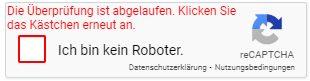
\includegraphics[width=6cm]{gfx/mygraphics/recaptchaabgelaufen.png}
     \caption{Zeitliche Begrenzung bei reCAPTCHA v2}
      \label{fig:recaptchaabgelaufen}
\end{figure}

\begin{table}[h!]
    \caption{Bewertungsmatrix CAPTCHAs mit minimalem User-Input}
    \begin{center}
        \begin{tabular}{l|c}
            Kategorie                       & Bewertung \\\hline
            Bedienfreundlichkeit            & 9         \\
            Accessibility                   & 10        \\
            Technische Umsetzbarkeit        & 10         \\
            Sicherheit                      & 8         
        \end{tabular}
    \end{center}
\end{table}

\subsection*{Zwischenfazit}
Während einige von ihnen, wie text-, audio- oder bildbasierte CAPTCHAs, noch oft verwendet werden, 
sind Methoden wie Gamification- oder videobasierte CAPTCHAs nur noch selten anzutreffen.
Doch werden auch Alternativen zu klassischen CAPTCHAs verwendet. Hier sind vor allem CAPTCHAs mit minimalem User-Input zu erwähnen. 